\documentclass[11pt,letterpaper]{article}

\usepackage{amsmath}
\usepackage{amssymb}
\usepackage{fancyhdr}
\usepackage{verbatim}
\usepackage{graphicx}


\oddsidemargin0cm
\topmargin-2cm
\textwidth16.5cm
\textheight23.5cm

\newcommand{\question}[1] {\vspace{.25in} \hrule\vspace{0.5em}
\noindent{\bf #1} \vspace{0.5em}
\hrule \vspace{.10in}}
\renewcommand{\part}[1] {\vspace{.10in} {\bf (#1)}}

\newcommand{\myname}{Karan Sikka}
\newcommand{\myandrew}{ksikka@cmu.edu}
\newcommand{\myhwnum}{01}

\setlength{\parindent}{0pt}
\setlength{\parskip}{5pt plus 1pt}

\pagestyle{fancyplain}
\lhead{\fancyplain{}{\textbf{HW\myhwnum}}}
\rhead{\fancyplain{}{\myname\\ \myandrew}}
\chead{\fancyplain{}{02-512}}

\begin{document}

\medskip

\thispagestyle{plain}
\begin{center}                  % Center the following lines
{\Large 02-512 Assignment \myhwnum} \\
\myname \\
\myandrew \\
\today
\end{center}

\question{1}
\part{a}
Cast problem as a bipartite graph where set A is the binding sites and B is the chemical groups.
Create edges such that edge between binding site and chemical group is the docking energy.
Now the problem is the Minimum Weight B-Perfect Matching (all vertices in B must be in the matching)


\part{b}
Create a graph where the vertices are the drugs and an edge connects drugs which may react with each other.
Now solve the Minimum Vertex Coloring problem. You can run all drugs (vertices) labeled with the same color at the same time. 
The problem minimizes the number of colors, which is the number of rounds.

\part{c}
Use the longest common subsequence pairwise on the sequences, allowing only for gaps. This is effective since the reads are long.
Keep track of the length of the common subsequence as a score between pairs. Then put the sequences in a graph as nodes where the edge weights are
the negatives of the scores obtained from LCS. Then use the traveling salesman problem to obtain the most likely original sequence.

\part{d}

Construct a graph where the nodes are the tissues and the edge weight for any $(v_1, v_2)$
is -1 x the probability that if the molecule is on tissue $v_1$ it will transport to $v_2$ (so that all edge weights are negative).
Then the problem can be considered as a single-pair shortest path problem where the start node is the start tissue and the end node is the target tissue.
The sum of the probabilities is minimized, which is not exactly what we want.

A better algorithm which suits the task (although not mentioned in class) is to start from the start node and traverse edge with the highest probability. If this results in a cycle, recurse on the neightbor connected by the next highest edge.
Otherwise you have traversed the path which the molecule is most likely to take. You could keep track of the path along the way and that would be the output of the algorithm.

\part{e}
Use longest common substring for $k$ strands obtained from the purified DNA strands. Do this for a small $k$ so that the probelm is tractable.
The substring found should be present in nearly every single strand, you can verify this in polynomial time. Otherwise choose a larger $k$ or resample $k$ strands.


\question{2}
\part{a}
Assume the input is a complete graph where the vertices are the labeled pixels and each edge has a weight equal to the euclidean distance between its vertices.
The output is a tree (undirected graph without cycles) covering all the vertices. Also known as a spanning tree.
The objective function is the sum of the edge weights of the tree, which we seek to minimize.

\part{b}
It's a minimum spanning tree problem. You can use Prim's algorithm.

2c.
Find the maximum $\Pi$ across all subsets of the nodes, where $\Pi$ is (sum of MST edges in subgraph with an added unlabeled vertex at the centroid of subgraph) - (sum of MST edges in subgraph)

2d.
Use a heuristic to quickly find a few points where the addition of an unlabeled vertex would be most beneficial.

2e.
When points are uniformly distributed the first algorithm works well.\\
When points are distributed unevenly, the second algorithm works better.


\question{3}
\part{a}
Here's the graph:\\

\begin{figure}[p]
    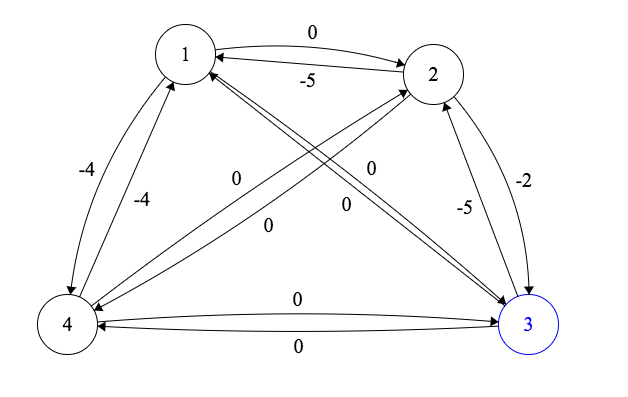
\includegraphics{3a.png}
\end{figure}

Adjacency matrix added for clarity.
\begin{verbatim}
       1  2  3  4
    1     0  0 -4
    2 -5    -2  0
    3  0 -5     0
    4 -4  0  0   
\end{verbatim}

\part{b}
The shortest path covering all vertices is \textless 3, 2, 1, 4 \textgreater.
Performing the alignment, we obtain the shortest common superstring:

    GTACGTTGTAATGTGCGCTAATG

\part{c}

First we split our sequences into 4-mers and 3-mers

\begin{verbatim}
1.
AATG, ATGT, TGTG, GTGC, TGCG, GCGC, CGCT
AAT, ATG, TGT, GTG, TGC, GCG, CGC, GCT

2.
CGTT, GTTG, TTGT, TGTA, GTAA, TAAT, AATG, ATGT
CGT, GTT, TTG, TGT, GTA, TAA, AAT, ATG, TGT

3.
GTAC, TACG, ACGT, CGTT, GTTG
GTA, TAC, ACG, CGT, GTT, TTG

4.
CGCT, GCTA, CTAA, TAAT, AATG
CGC, GCT, CTA, TAA, AAT, ATG
\end{verbatim}

Now we construct a graph where nodes are k-1 mers and edges represent the presence of k mers

\begin{verbatim}
Nodes:
AAT, ACG, ATG, CGC, CGT, CTA, GCG, GCT, GTA, GTG, GTT, TAA, TAC, TGC,
TGT, TTG

Edges:
AAT -> ATG (AATG)
ACG -> CGT (ACGT)
ATG -> TGT (ATGT)
CGC -> GCT (CGCT)
CGT -> GTT (CGTT)
CTA -> TAA (CTAA)
GCG -> CGC (GCGC)
GCT -> CTA (GCTA)
GTA -> TAA (GTAA)
GTA -> TAC (GTAC)
GTG -> TGC (GTGC)
GTT -> TTG (GTTG)
TAA -> AAT (TAAT)
TAC -> ACG (TACG)
TGC -> GCG (TGCG)
TGT -> GTA (TGTA)
TGT -> GTG (TGTG)
TTG -> TGT (TTGT)
\end{verbatim}


No unique solution because there is a cycle and you could include any number of cycle iterations in the resulting eulerian path.\\
\verb!TAA -> AAT -> ATG -> TGT -> GTA -> TAA ...!

\part{d}
First we split our sequences into 5-mers and 4-mers
\begin{verbatim}
1.
AATGT, ATGTG, TGTGC, GTGCG, TGCGC, GCGCT
AATG, ATGT, TGTG, GTGC, TGCG, GCGC, CGCT

2.
CGTTG, GTTGT, TTGTA, TGTAA, GTAAT, TAATG, AATGT
CGTT, GTTG, TTGT, TGTA, GTAA, TAAT, AATG, ATGT

3.
GTACG, TACGT, ACGTT, CGTTG
GTAC, TACG, ACGT, CGTT, GTTG

4.
CGCTA, GCTAA, CTAAT, TAATG
CGCT, GCTA, CTAA, TAAT, AATG

Nodes:
AATG, ACGT, ATGT, CGCT, CGTT, CTAA, GCGC, GCTA, GTAA, GTAC, GTGC,
GTTG, TAAT, TACG, TGCG, TGTA, TGTG, TTGT

Edges:
AATG -> ATGT (AATGT)
ACGT -> CGTT (ACGTT)
ATGT -> TGTG (ATGTG)
CGCT -> GCTA (CGCTA)
CGTT -> GTTG (CGTTG)
CTAA -> TAAT (CTAAT)
GCGC -> CGCT (GCGCT)
GCTA -> CTAA (GCTAA)
GTAA -> TAAT (GTAAT)
GTAC -> TACG (GTACG)
GTGC -> TGCG (GTGCG)
GTTG -> TTGT (GTTGT)
TAAT -> AATG (TAATG)
TACG -> ACGT (TACGT)
TGCG -> GCGC (TGCGC)
TGTA -> GTAA (TGTAA)
TGTG -> GTGC (TGTGC)
TTGT -> TGTA (TTGTA)
\end{verbatim}

Yes, there is a unique solution. An eulerian path must start with an odd-degree vertex and there are only two. Only one of the two leads to an eulerian path.

\part{e}
\begin{verbatim}
GTAC -> TACG (GTACG)
TACG -> ACGT (TACGT)
ACGT -> CGTT (ACGTT)
CGTT -> GTTG (CGTTG)
GTTG -> TTGT (GTTGT)
TTGT -> TGTA (TTGTA)
TGTA -> GTAA (TGTAA)
GTAA -> TAAT (GTAAT)
TAAT -> AATG (TAATG)
AATG -> ATGT (AATGT)
ATGT -> TGTG (ATGTG)
TGTG -> GTGC (TGTGC)
GTGC -> TGCG (GTGCG)
TGCG -> GCGC (TGCGC)
GCGC -> CGCT (GCGCT)
CGCT -> GCTA (CGCTA)
GCTA -> CTAA (GCTAA)
CTAA -> TAAT (CTAAT)
\end{verbatim}

Shortest string consistent with graph: GTACGTTGTAATGTGCGCTAAT

No it's not the same as the TSP solution. It's missing one character at the end.
This disparity is because we lost some information when breaking the sequence apart into 5-mers, increasing the ambiguity when reassembling the pieces.
The result of this method was a shorter string, which agreed with the 5-mer data but not completely with the original 4 longer sequences.

\question{4}
\part{a}
Input is a set of drugs, and a set of pairs of drugs which are toxic when taken together.
Output is a list of drugs which are not toxic when taken together.
Objective function is the length of the output list, which we will maximize.

\part{b}
This is similar to the Maximum Independent Set problem, if the drugs are vertices and there's an edge between two drugs which interact toxically.

\part{c}

\begin{verbatim}
function getMaxIndSet(drugs, interact)
    max_set = {}
    if size(drugs) == 0:
        return {}
    For every drug d1 in drugs:
        ind_set_with_d1 = {d1} + getMaxIndSet(drugs
                     - {d1}
                     - {d2 for d2 in drugs if (d1, d2) interact}))
        ind_set_without_d1 = getMaxIndSet(drugs - {d1})

        if size(ind_set_with_d1) > size(max_set):
            max_set = ind_set_with_d1

        if size(ind_set_without_d1) > size(max_set):
            max_set = ind_set_without_d1

    return max_set
\end{verbatim}

\part{d}
Written in Python 2.7:\\
\verbatiminput{mis.py}

\part{e}
On the first input, the program outputs ``0 2 4".\\
On the second input, the program outputs ``0 3 5".\\


\end{document}
